\title{INTD262: Science or Not Science?}
\author{Dr. Jordan Hanson - Whittier College Dept. of Physics and Astronomy}
\date{\today}
\documentclass[12pt]{article}
\usepackage[margin=1.5cm]{geometry}
\usepackage{hyperref}
\usepackage{graphicx}
\usepackage{amsmath}
\begin{document}
\maketitle

\section{Introduction}

In this activity, we will attempt to classify fields of knowledge scientifically.  Recall that in the introduction and chapter 1 of \textit{The Scientific Attitude}, we find a discussion about the difference between subjects that are \textit{scientific}, and \textit{non-scientific}.  The \textit{non-scientific} category may be split into two categories: \textit{humanistic} and \textit{pseudo-scientific}.  Fields in the former category are not meant to be forms of scientific inquiry (literature, history, languages).  The second sub-category contains fields that \textit{impersonate} science.  Examples of pseudo-science include astrology, creationism, and the link between vaccines and autism.  In this activity, we will examine synopses of fields of inquiry, and use the synopses to classify the fields as scientific, humanistic, or pseudo-scientific.  The goal of this exercise is to practice making the distinction between fields that are theoretically warranted and backed by voluminous empirical evidence, those that have neither, and humanistic fields we value for reasons beyond the scope of science.

\section{Classification: Science vs. Non-Science and Science vs. Pseudo-Science}

\begin{figure}[h]
\centering
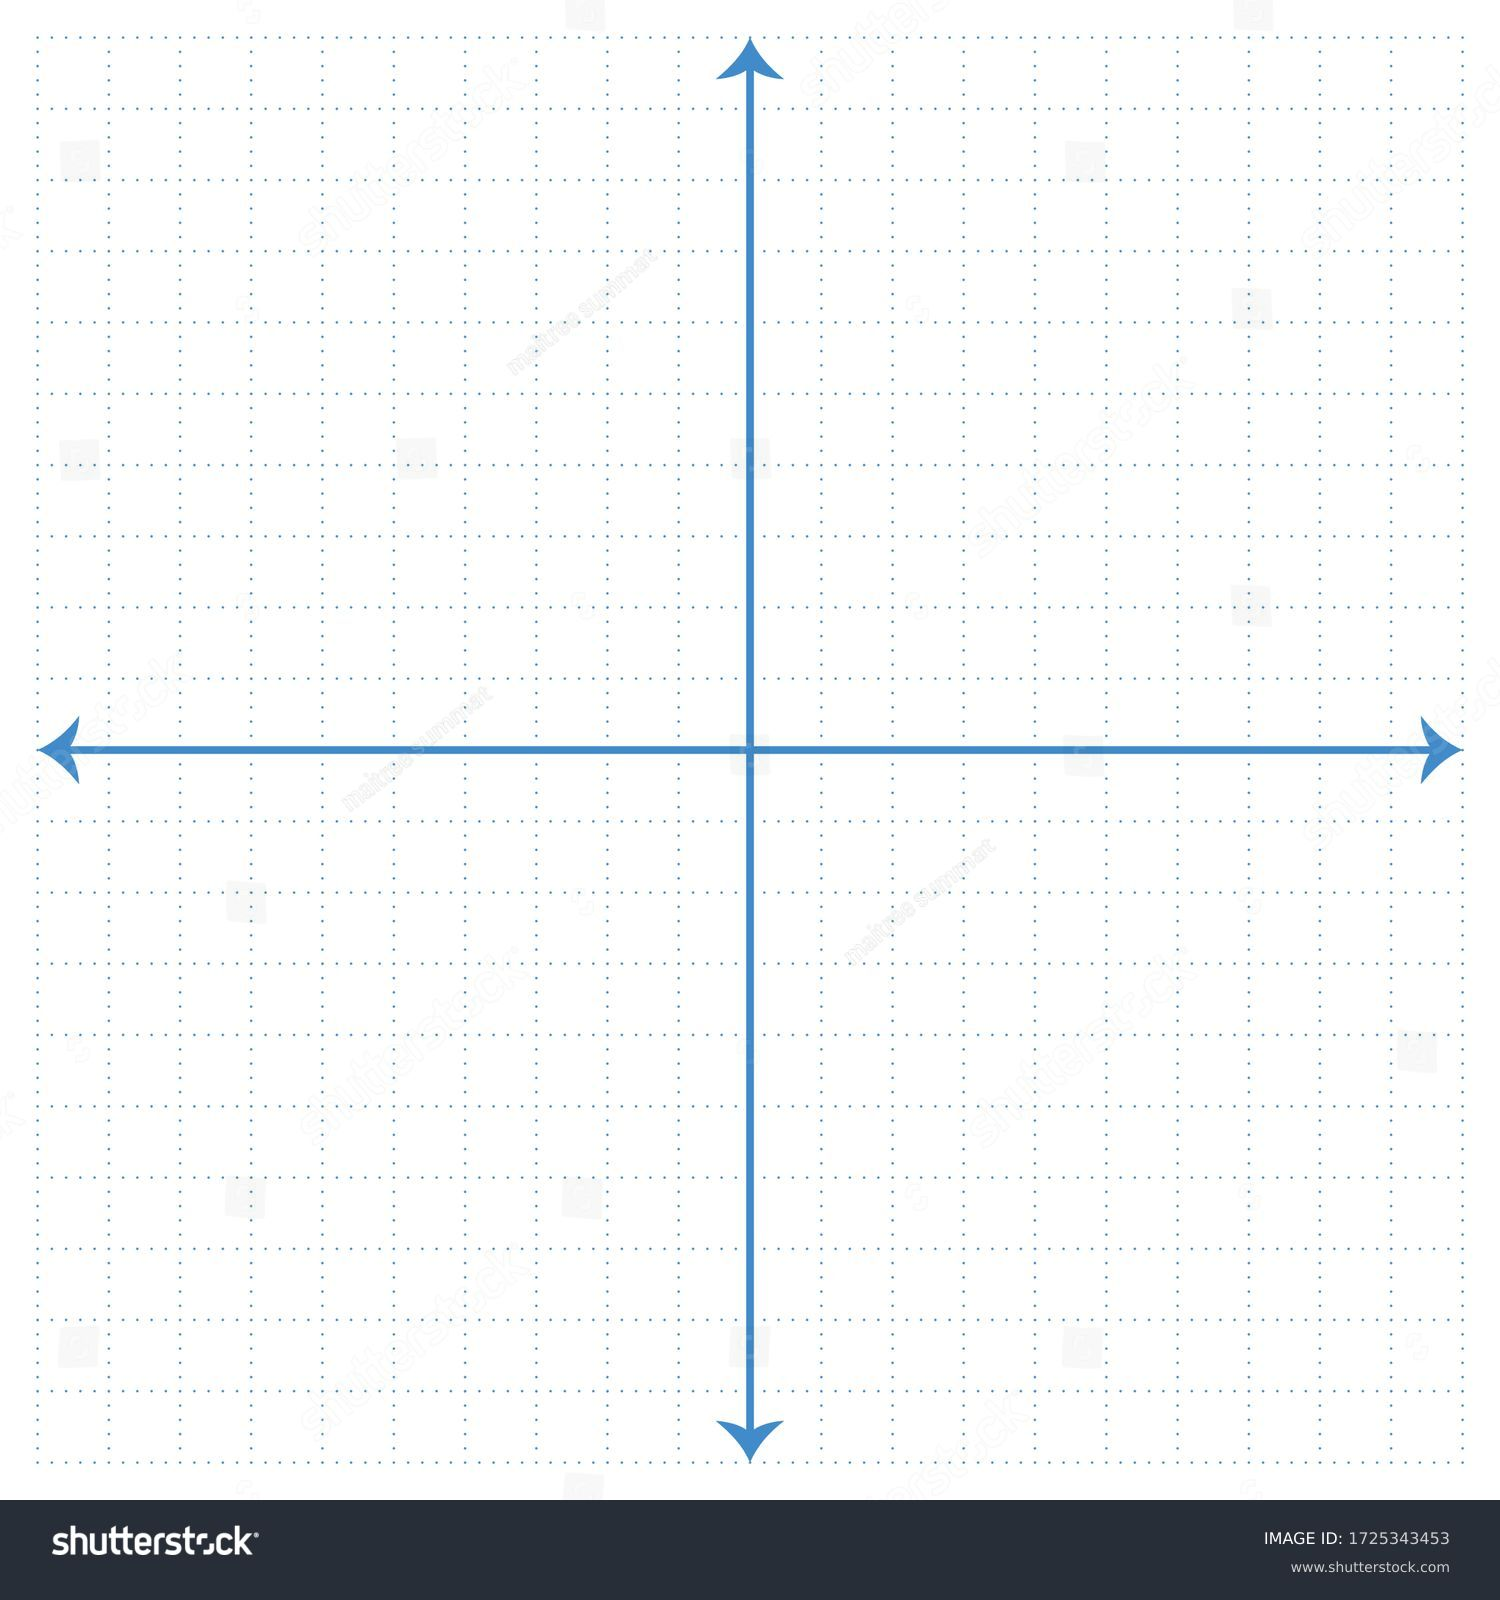
\includegraphics[width=0.4\textwidth,trim=0cm 3.6cm 0cm 0cm,clip=true]{figures/graph.jpg}
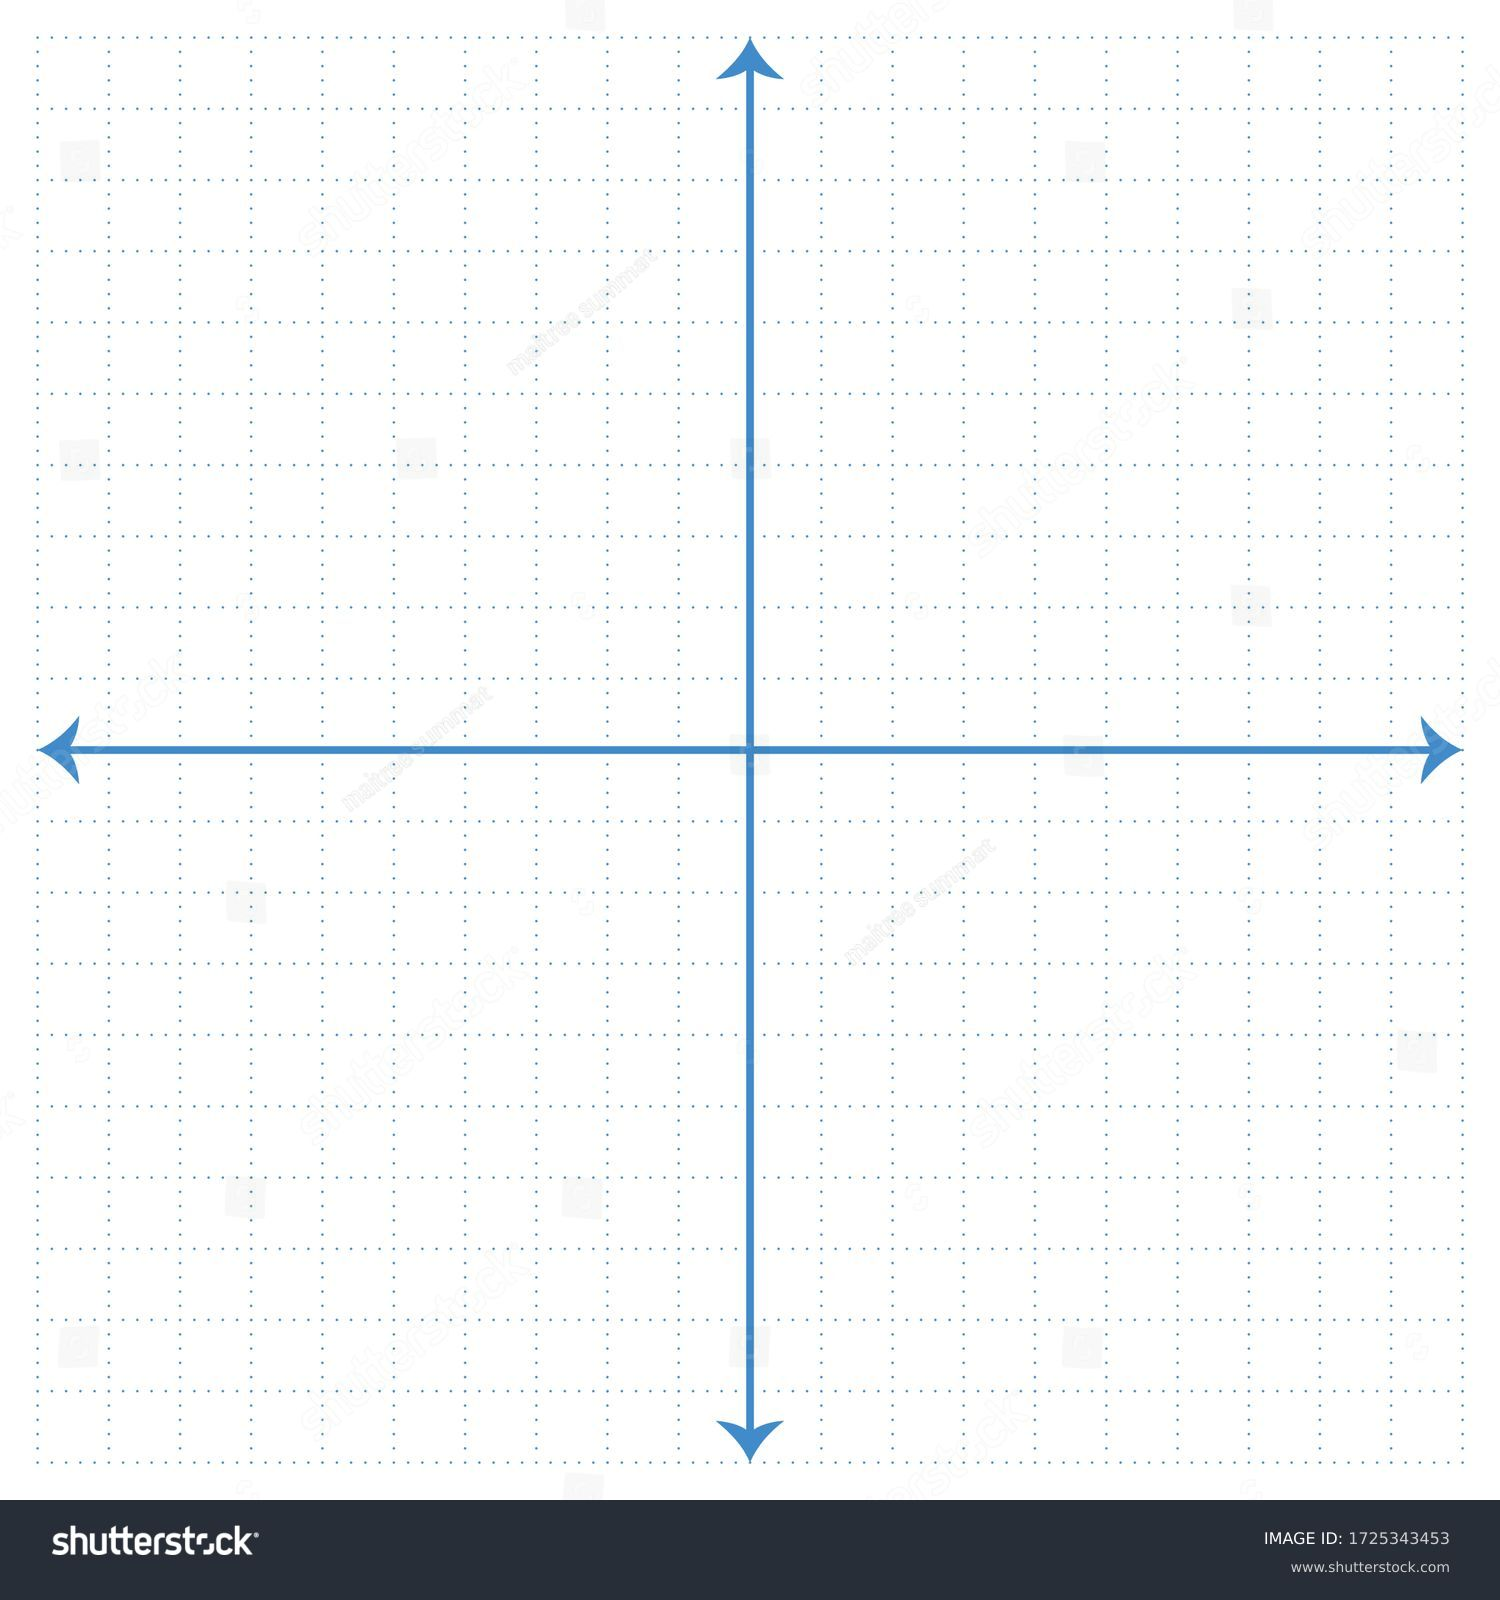
\includegraphics[width=0.4\textwidth,trim=0cm 3.6cm 0cm 0cm,clip=true]{figures/graph.jpg}
\caption{\label{fig:1} (Left) \textbf{Science and Non-Science.} Label the positive x-axis of the left graph ``empirical,'' and the negative x-axis of the left graph ``non-empirical.''  Label the positive y-axis of the left graph ``natural,'' and the negative y-axis ``human origin.''  (Right) \textbf{Science and Pseudo-science.} Label the positive x-axis and y-axis of the right graph ``falsifiable'' and ``theoretical,'' respectively.}
\end{figure}

\section{Synopses of a Variety of Fields}

Upon reading a synopsis of a field of inquiry below, first make an attempt to place it within the 2D space of Fig. \ref{fig:1} (left).  If the location of the field is sufficiently within the upper-right quadrant of Fig. \ref{fig:1} (left), make an attempt to place it within the 2D space of Fig. \ref{fig:1} (right).

\subsection{Philosophy}

Modern philosophy (late 1500s - 1900s) marks a significant shift from traditional scholasticism to a focus on reason, individualism, and the nature of knowledge. Key figures such as Ren\'{e} Descartes emphasized the importance of doubt and the use of reason as a path to certainty. This period saw the rise of empiricism, led by philosophers like Locke and Hume, who argued that knowledge comes primarily from sensory experience. Concurrently, rationalism, represented by thinkers like Spinoza and Leibniz, posited that reason is the primary source of knowledge. Kant's critical philosophy later sought to reconcile these opposing views by exploring the limits and conditions of human understanding. The era also gave birth to existentialism, phenomenology, and analytic philosophy, which further explored human existence, consciousness, and language, fundamentally shaping contemporary thought.

\subsection{Classical Physics}

Classical physics (late 1600s - 1800s) encompasses the foundational theories that describe the macroscopic physical world. Rooted in the work of Isaac Newton, whose laws of motion and universal gravitation provided a comprehensive framework for understanding the movement of objects, classical physics explains phenomena such as force, energy, and momentum, and electromagnetism.  The latter is formulated with Maxwell's equations, which describe how electric and magnetic fields interact and propagate as electromagnetic waves. Additionally, thermodynamics emerged, governing the principles of energy transfer and the temperature-dependent behavior of systems. Classical physics successfully explained a wide range of physical phenomena and laid the groundwork for engineering, astronomy, and technology.

\subsection{Modern Physics}

Modern physics, emerging in the early 20th century, represents a profound departure from classical physics, addressing phenomena that classical theories could not explain. It is primarily defined by two groundbreaking theories: quantum mechanics and relativity. Quantum mechanics explores the behavior of matter and energy at the atomic and subatomic levels, introducing concepts such as wave-particle duality, quantization, and the uncertainty principle. Meanwhile, the theory of relativity, encompassing both special and general relativity, revolutionized our understanding of space, time, and gravity, demonstrating that time and space are interconnected and relative, not absolute. Modern physics also includes advancements in particle physics, cosmology, and condensed matter physics, significantly expanding our understanding of the universe, from the smallest particles to the vastness of space.

\subsection{Mexican Herbal Medicine}

Mexican herbal medicine is a deeply rooted tradition that blends indigenous knowledge with influences from Spanish colonialism and African cultures, creating a rich tapestry of healing practices. Indigenous groups such as the Aztecs, Maya, and Zapotecs have long relied on a wide variety of plants for medicinal purposes, using herbs like epazote for digestive issues, tepezcohuite for skin conditions, and damiana for reproductive health. These practices are often intertwined with spiritual beliefs, where healers, known as curanderos, use rituals alongside herbal remedies to treat both physical and spiritual ailments. Relying on diverse flora, this tradition reflects a deep connection to the land and has been passed down through generations to our time. As interest in natural and holistic healing grows, Mexican herbal medicine is gaining recognition for its effectiveness and is increasingly being studied in a modern context.

\subsection{Political Science in the United States}

American political science (late 1800s - today) is a field dedicated to the systematic study of politics, government, and political behavior within the United States. It evolved alongside the development of American political institutions and democracy. The discipline encompasses the analysis of political theory, institutions like Congress, the Presidency, and the Supreme Court, as well as electoral systems, public opinion, and policy-making processes. Scholars in American political science examine the functioning of federalism, the role of political parties, and the impact of interest groups and the media on governance. The field also explores broader themes such as democracy, representation, and civil rights, often focusing on the balance between liberty and equality. As a dynamic discipline, it employs a variety of methodologies, including qualitative case studies, quantitative analysis, and comparative approaches, to understand and predict political trends and outcomes in the USA.

\subsection{Chemistry}

Chemistry is an exploration of the properties, composition, and behavior of matter, focusing on the interactions and transformations of substances at the atomic and molecular levels. It serves as a bridge between the physical and life sciences, playing a crucial role in understanding the material world and the processes that govern it. Chemistry is divided into various branches.  Organic and inorganic chemistry separate the study of substance that do or do not contain carbon.  Physical chemistry combines physics and chemistry to understand how matter behaves.  Analytical chemistry is the study of identifying and quantifying substances.  The field has wide-ranging applications, including new materials, medicines, new energy solutions, and understanding biological and environmental process. Central concepts in chemistry include atomic structure, chemical bonding, and reaction mechanisms.

\subsection{Mayan Astronomy}

Mayan astronomy was a sophisticated and integral aspect of the ancient Maya civilization, reflecting their deep understanding of celestial bodies and their movements. The Maya meticulously observed the stars, planets, and cycles of the sun and moon, using this knowledge to develop a highly accurate calendar system that included the 260-day Tzolk'in and the 365-day Haab'. Their observations were crucial for agricultural planning, religious ceremonies, and political events, as the Maya believed that the heavens directly influenced earthly affairs. Mayan astronomers built observatories, such as the famous El Caracol in Chichén Itzá, to track celestial events like solstices, equinoxes, and eclipses. Their knowledge was recorded in codices and inscribed on monuments, demonstrating an advanced understanding of astronomical cycles, including the Venus cycle, which was particularly significant in their cosmology. The Maya's integration of astronomy with their religious and cultural life highlights the importance they placed on understanding and aligning with the cosmos.

\subsection{Religious Studies}

Religious studies in American universities is an interdisciplinary field that explores the diversity of religious beliefs, practices, and institutions across cultures and throughout history. Religious studies adopts a neutral, comparative approach, examining religions as social, cultural, and historical phenomena. The curriculum typically includes the study of major world religions like Christianity and Judaism, Islam, Hinduism, Buddhism, and indigenous religious movements. Courses often cover themes such as mythology, ethics, ritual, sacred texts, and the role of religion in politics and society. Students are encouraged to critically analyze the ways religion shapes and is shaped by culture, identity, and power dynamics. The field draws on methods from anthropology, sociology, history, psychology, and philosophy, fostering a broad, inclusive understanding of the complex role religion plays in human experience.

\subsection{Economics}

Economics is the study of how societies allocate scarce resources to meet the needs and wants of individuals and businesses, aiming to understand and improve decision-making processes in both microeconomic and macroeconomic contexts. Microeconomics focuses on the efficiency of individuals and businesses, including the study of market mechanisms, supply and demand, and pricing strategies. Macroeconomics, on the other hand, examines broader economic phenomena such as national income, inflation, unemployment, and economic growth, seeking to develop policies to stabilize and stimulate the economy. The field incorporates various theoretical models to explain and predict outcomes, including classical, Keynesian, and contemporary approaches. Economics also intersects with other disciplines, such as political science, sociology, and environmental science.

\subsection{Incan Mathematics}

Incan mathematics, developed by the Inca Empire prior to European contact, was an advanced system adapted to their societal needs and environment. Central to Incan mathematics was the use of \textit{quipus}, a system of knotted strings that encoded numerical data that enabled complex record-keeping and administrative functions. Although the Inca did not use a written numerical system, their mathematics was highly practical, focusing on concepts like measurement, accounting, and agriculture. They employed base-10 and base-60 systems for calculations and had a sophisticated understanding of geometric and spatial relationships.  These concepts were essential for their engineering feats, such as building extensive road networks and agricultural terraces. Incan mathematicians were skilled in practical arithmetic and geometry, which they used to manage trade, construction, and taxation within their vast empire.

\section{Conclusion}

Our goal is to develop a nuanced understanding of the demarcation between fields.  Our individual versions of Fig. \ref{fig:1} will depend on our perspective.  Our individual versions, however, should be correlated.

\begin{figure}[hb]
\centering
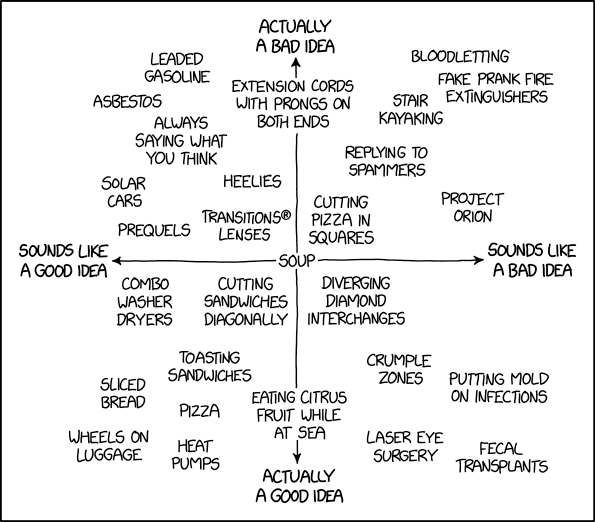
\includegraphics[width=0.35\textwidth]{figures/good_and_bad_ideas.png}
\caption{\label{fig:2} Sliced bread is objectively a good idea. (Credit: \url{xkcd.com}).}
\end{figure}

\end{document}
